\vspace{-0.7cm}
\section{Introduction}
\label{sec:intro}
Large language models (LLMs)~\cite{wei2022emergent, openai2024gpt4technicalreport,deepseekai2025deepseekv3technicalreport} are rapidly transforming modern computing, powering applications such as conversational assistants~\cite{dam2024completesurveyllmbasedai,10.1145/3580305.3599572}, code generation~\cite{hui2024qwen25codertechnicalreport}, and retrieval-augmented generation~\cite{NEURIPS2020_6b493230,yao2025cacheblendfastlargelanguage}. As these models transition from research to production, cloud AI engines~\cite{openai2024chatgpt,anthropic2024claude,google2024gemini} must improve serving latency and resource efficiency for both online and offline inference. While prior work has proposed scheduling strategies~\cite{pang2025optimizing,zhong2024distservedisaggregatingprefilldecoding,zheng2025bucketservebucketbaseddynamicbatching,agrawal2024tamingthroughputlatencytradeoffllm}, parallelization techniques~\cite{su2025seesawhighthroughputllminference,wu2024loongserveefficientlyservinglongcontext}, memory management methods~\cite{kwon2023efficient,prabhu2025vattentiondynamicmemorymanagement,zhang2025jengaeffectivememorymanagement}, quantization~\cite{chee2024quip2bitquantizationlarge,lin2024awqactivationawareweightquantization}, and kernel-level optimizations~\cite{yi2026pat,MLSYS2025_96894468}, efficiently serving LLM workloads, especially under realistic high-throughput conditions, remains an open problem.

\begin{figure}[t]
\captionsetup[subfigure]{labelformat=simple}
    \renewcommand\thesubfigure{(\alph{subfigure})}
\centering
\begin{subfigure}{0.55\columnwidth}
    \centering
    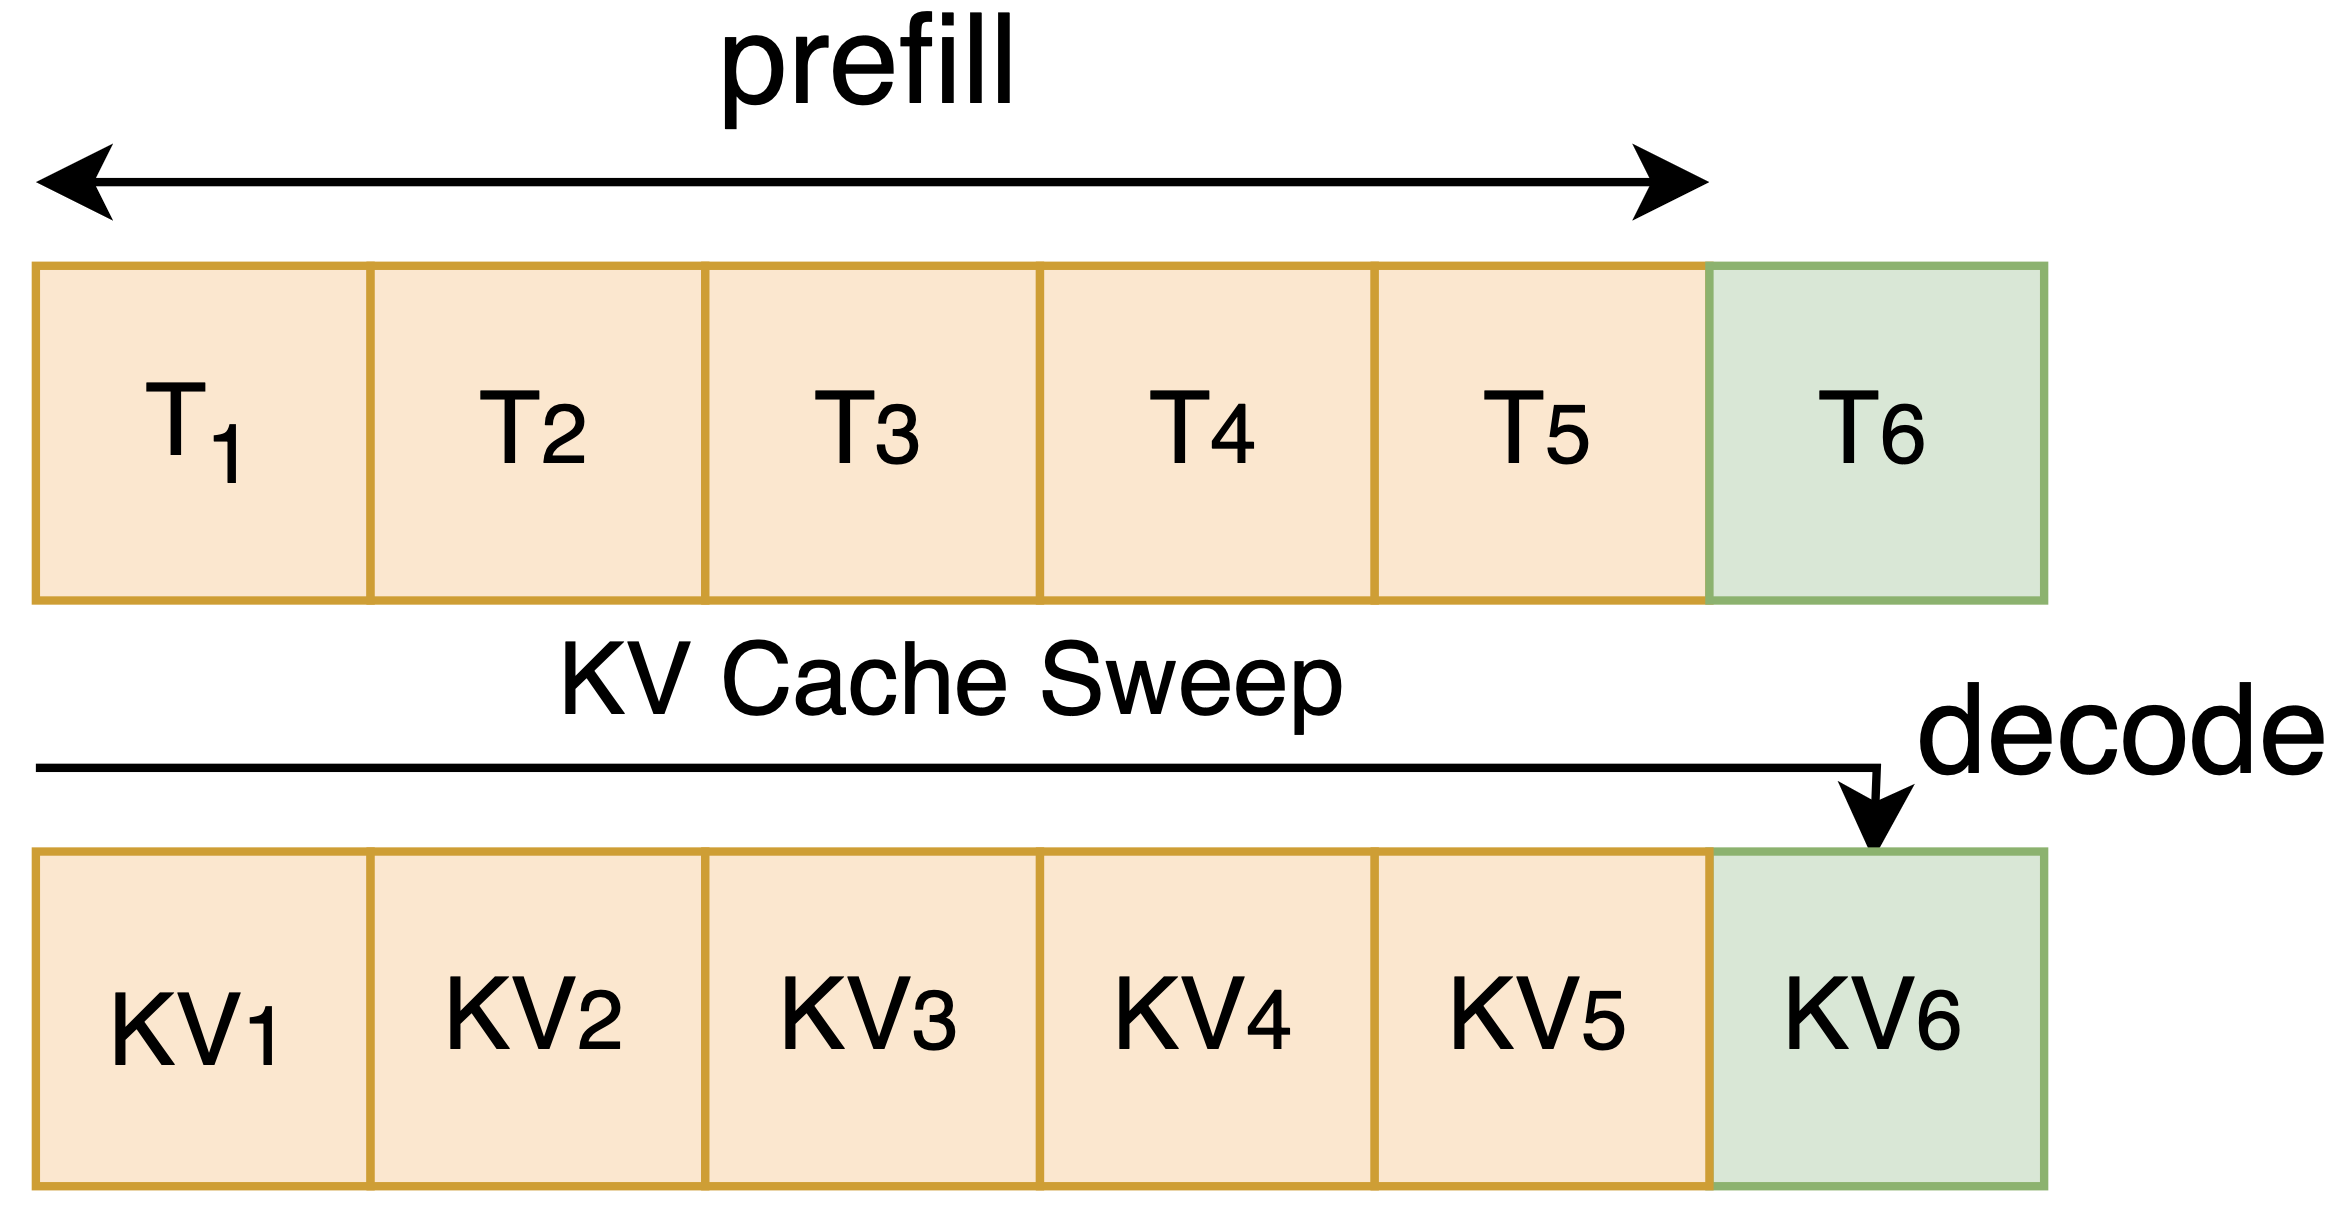
\includegraphics[width=\linewidth]{illustration_images/prefill_decode.png}
    \caption{Prefill and Decode}
    \label{fig:prefill_decode}
\end{subfigure}
\hspace{5pt}
\begin{subfigure}{0.25\columnwidth}
    \centering
    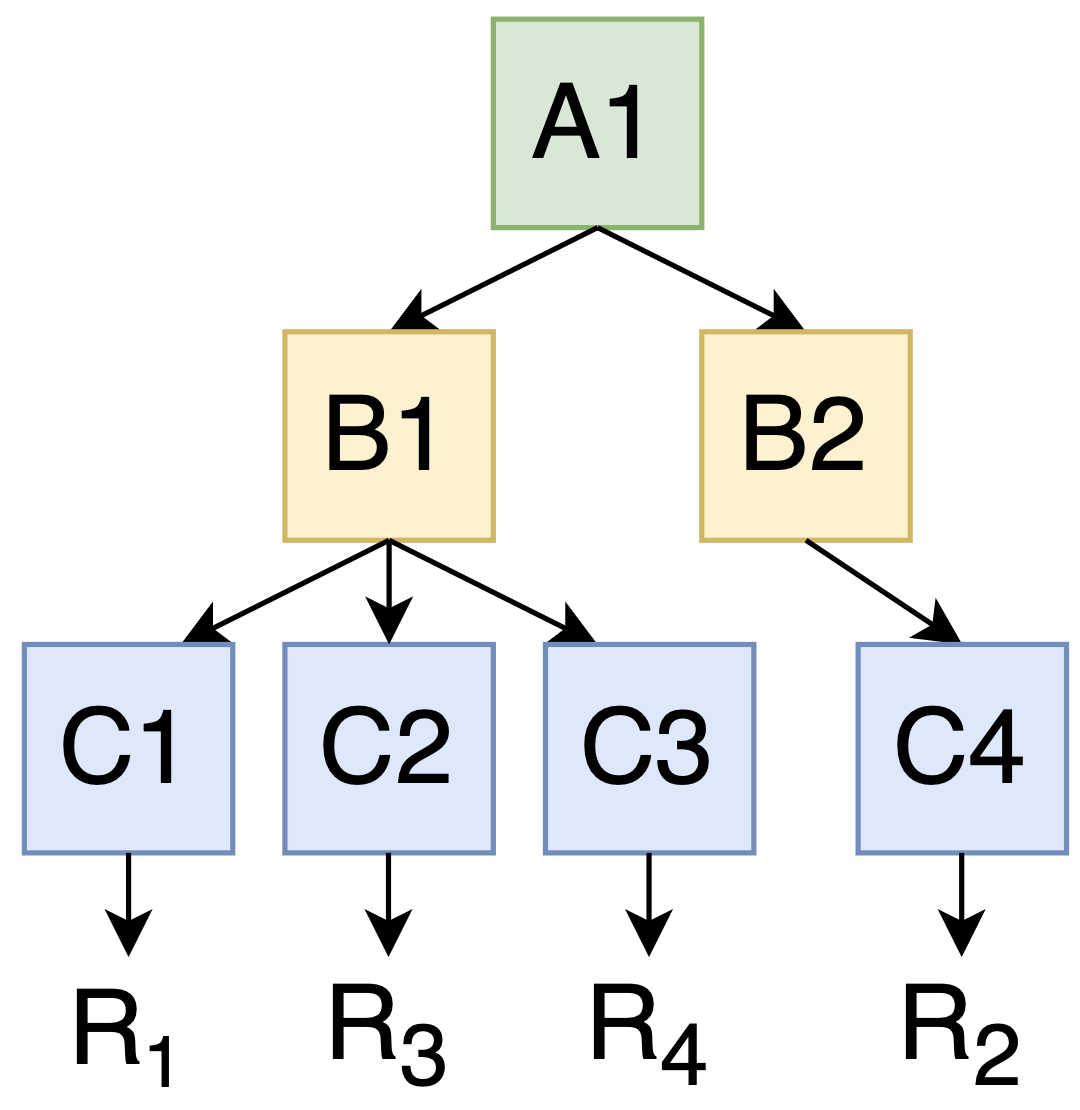
\includegraphics[width=\linewidth]{illustration_images/radix_tree.png}
    \caption{Radix Tree}
    \label{fig:radix_tree_four_requests}
\end{subfigure}
\caption{LLM Inference Primitives}
\label{fig:prefill_decode_radix_tree}
\vspace{-15pt}
\end{figure}

An LLM inference request goes through two phases: \textit{prefill} and \textit{decode}. The prefill phase processes all prompt tokens in parallel to produce the first output token, making it compute-bound. The decode phase, by contrast, generates tokens auto-regressively and is fundamentally memory-bound. 
Each newly generated token attends to the keys and values of all previous tokens, resulting in a sweep of the entire KV cache for each decode iteration, as shown in Figure~\ref{fig:prefill_decode}. As context lengths grow, this memory traffic becomes the dominant bottleneck. 
Popular LLM inference engines like vLLM~\cite{kwon2023efficient} adopt batching to improve GPU utilization during the decode phase, scheduling multiple requests together in a batch using policies like First Come First Serve (FCFS). More advanced frameworks explore techniques such as interleaving~\cite{agrawal2024tamingthroughputlatencytradeoffllm}, disaggregation~\cite{zhong2024distservedisaggregatingprefilldecoding}, and spatial co-scheduling~\cite{Kamath_2025,lin2025boostingllmservingspatialtemporal}, along with dynamically adjusting batch sizes based on runtime constraints~\cite{pang2025optimizing}, to address this compute-memory mismatch. 

Orthogonally, workloads such as few-shot prompting~\cite{brown2020languagemodelsfewshotlearners,NEURIPS2021_5c049256}, system prompts~\cite{thebigpromptlibrary}, and RAG~\cite{lewis2021retrievalaugmentedgenerationknowledgeintensivenlp} exhibit significant \textit{prefix sharing} across requests. Reusing KV caches for shared prefixes eliminates redundant KV computation and reduces memory footprint. Systems such as SGLang~\cite{zheng2024sglangefficientexecutionstructured} and vLLM \cite{kwon2023efficient} use radix trees (Figure~\ref{fig:radix_tree_four_requests}) or hashing-based structures to keep track of shared KV caches. While vLLM's FCFS would have scheduled requests in arrival order ($R_1, R_2, R_3, R_4$), SGLang performs a depth-first traversal of the radix tree and schedules requests in the order $R_1, R_3, R_4, R_2$, which reduces KV cache evictions.
A complementary line of work~\cite{yi2026pat,yao2025deftdecodingflashtreeattention,ye2024chunkattentionefficientselfattentionprefixaware,MLSYS2025_96894468} exploits the shared prefix structure within the attention kernel itself by jointly computing attention for groups of queries that share prefixes. Such prefix-aware attention kernels avoid redundant loading of shared KV blocks for each request separately, thereby reducing memory traffic. 

Despite these advances, we identify two critical gaps in current scheduling strategies for prefix-shared workloads. First, prior work largely focuses on maximizing batch size during the decode phase. However, we show via controlled experiments that prefix homogeneity — the extent to which \textit{all} requests in a batch share a common prefix — has an even stronger impact on performance. Further, we find that the performance gains increase with the length of the prefix shared across all the requests in a batch (\S\ref{subsec:significance_of_prefix_homogeneity}). This is because when a prefix is shared by all requests, there is significant \textit{spatial} and \textit{temporal} locality in the memory accesses of the KV cache located in the GPU DRAM, which leads to both higher memory bandwidth utilization and reduced total amount of data fetched from DRAM. As a result, moderately small prefix-homogeneous batches can leverage these locality benefits and perform better than larger heterogeneous batches. For example, Figure~\ref{fig:prefill_decode_homo_hetero_grouped_throughput_tok100} shows the throughput and execution times of 800 requests, where 8 groups of 100 requests each share a large prefix of 10K tokens between them. Processing these requests in 8 prefix-homogeneous batches of 100 requests each leads to nearly 2$\times$ higher throughput than when using larger heterogeneous batches, though very small homogeneous batches (32 batches of 25 requests each) perform poorly as well due to sub-optimal compute utilization. Existing prefix-aware schedulers have no mechanism to recognize this tradeoff between batch size and prefix homogeneity (\S\ref{subsec:batch_size_vs_prefix_homogeneity}); e.g., in Figure~\ref{fig:radix_tree_four_requests}, a DFS-traversal-based scheduler will use $R_2$ to maximize batch size, even if a smaller batch (only $R_1, R_3, R_4$) could have performed better due to a longer common prefix. The second big gap with current prefix-aware schedulers is that they incur prohibitive CPU overheads in maintaining and traversing radix trees, which can account for 50–90\% of total latency (\S\ref{subsec:overhead_dynamic_prefix_detection}). 

\begin{figure}[t]
  \centering
  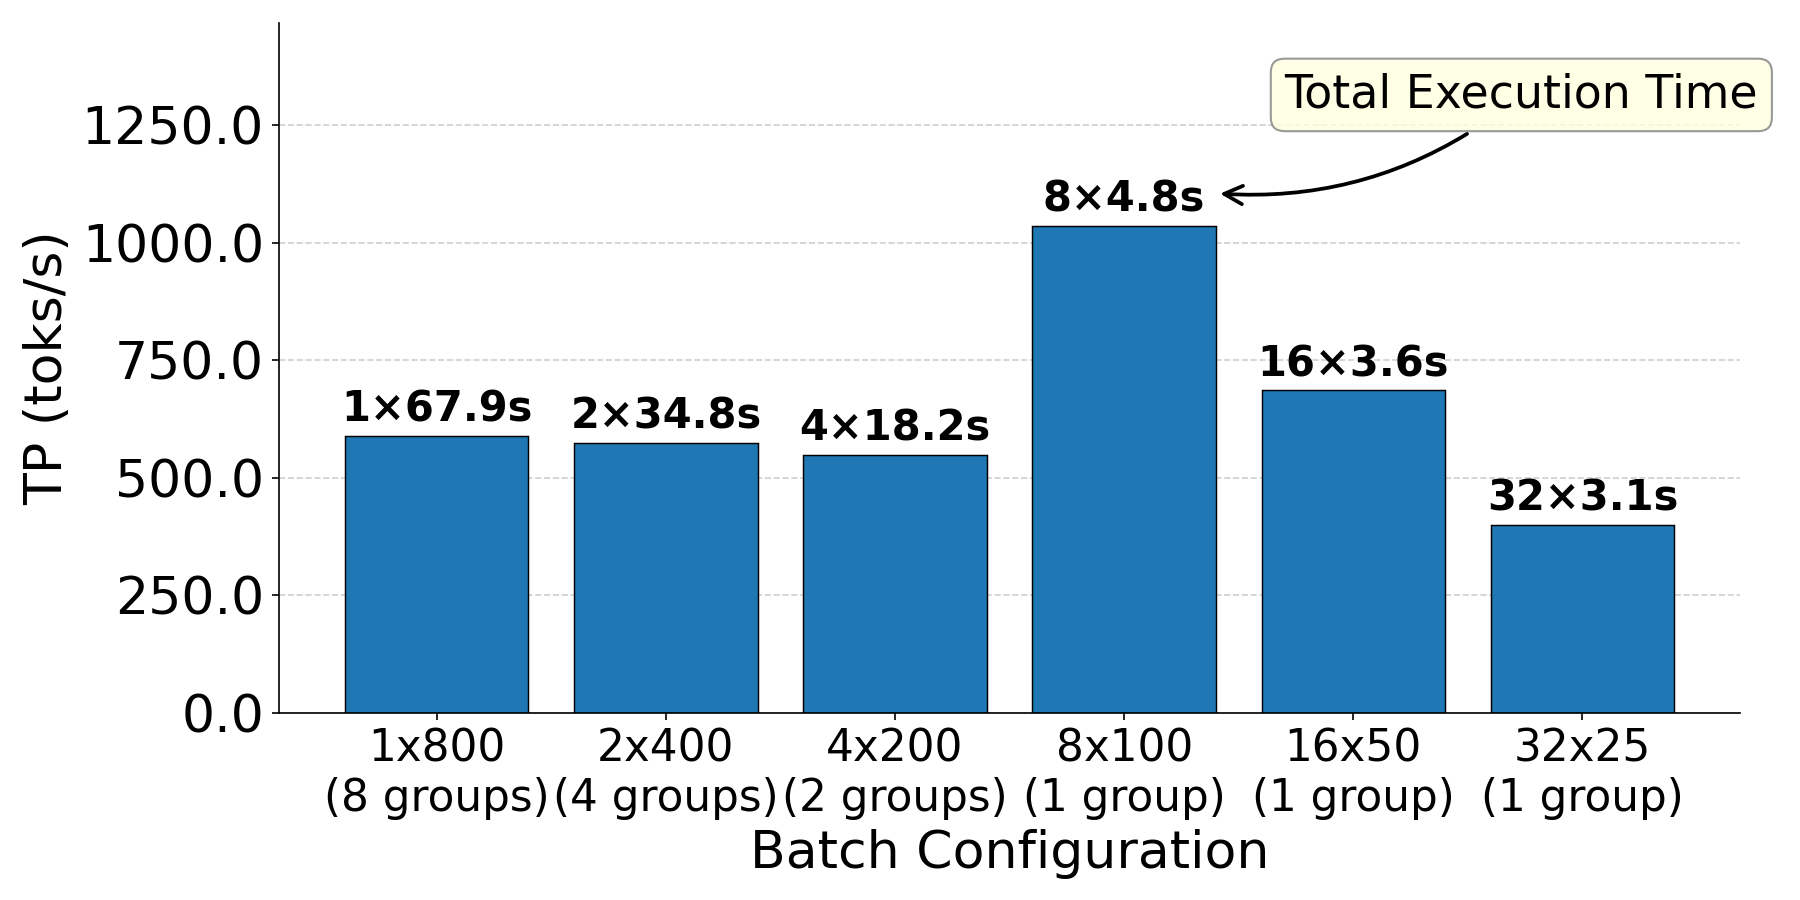
\includegraphics[width=0.75\linewidth]{results/prefill_decode_homo_hetero_grouped_throughput_tok100.png}
  \captionsetup{skip=2pt}
  \caption{Batch Size vs. Prefix Homogeneity}
  \label{fig:prefill_decode_homo_hetero_grouped_throughput_tok100}
  \vspace{-20pt}
\end{figure}

This paper introduces \Feather\footnote{Please see \S\ref{sec:about_feather} for an explanation of this name.} (\S\ref{sec:design}), a prefix-aware scheduler that improves throughput by efficiently finding an optimal balance between batch size and prefix homogeneity. \Feather is built on two components: \textit{(i) Chunked Hash Tree (CHT)}, a lightweight data structure for fast prefix detection, similar in spirit to vLLM's block table~\cite{kwon2023efficient}. Instead of performing token-level radix tree traversals, CHT represents each request as a vector of cumulative prefix hashes. To efficiently select a request that maximizes the length of the prefix shared across the active batch, CHT maintains a \textit{min-heap}, updated lazily, and ordered by per-request \textit{missing count}---the number of prefix chunks not yet covered by the batch. This enables the identification of the best candidate in $\mathcal{O}(\log W)$ time among $W$ waiting requests, a significant improvement over DFS traversal~\cite{zheng2024sglangefficientexecutionstructured}. \textit{(ii) RL-based batching policy}. Deciding when to stop adding requests to a batch presents a trade-off: larger batches improve utilization but dilute prefix homogeneity. We cast this as a reinforcement learning problem in which the scheduler observes batch characteristics (e.g., current size, shared prefix length), evaluates the impact of adding another request to the batch, and stops batch formation at a point that maximizes throughput. This adaptive approach consistently outperforms static heuristics across diverse workloads and hardware configurations. Together, these two components enable \Feather to construct prefix-homogeneous batches efficiently, both improving system throughput and reducing scheduling overhead.

We implement \Feather on vLLM~\cite{kwon2023efficient} and SGLang~\cite{zheng2024sglangefficientexecutionstructured} and evaluate it across diverse workloads and configurations (\S\ref{sec:eval}). Our results show that \Feather achieves $2$-$10\times$ higher end-to-end throughput over vLLM's FCFS and other baselines for shared prefix lengths ranging from 1K to 10K tokens, while also improving DRAM bandwidth utilization. \Feather is fully hardware-agnostic and yet performs better than recent prefix-aware kernels that must be tuned to specific hardware configurations. 
Our RL policy ensures that our performance never falls below that of the baselines, even if the workload does not allow for prefix-homogeneous batches, and CHT reduces prefix-detection overhead by up to $1000\times$ compared to DFS-based approaches for long sequences. 

In summary, this paper makes the following contributions: (i) We demonstrate the tradeoff between batch size and prefix homogeneity in the decode phase performance of LLM inference, and identify previously overlooked CPU overheads in prefix-aware scheduling. (ii) We design the Chunked Hash Tree (CHT) data structure for low-overhead prefix detection, and develop a reinforcement learning-based policy for adaptive batch construction. (iii) We build \Feather, a prefix-aware scheduler integrated into vLLM and SGLang, and demonstrate improvements in throughput and latency on diverse workloads. We plan to open-source \Feather by contributing it to both frameworks' repositories.